\documentclass[aps,prb,twocolumn,nofootinbib,superscriptaddress]{revtex4-2}
\usepackage{amsmath,amssymb,graphicx,booktabs}
\usepackage[T1]{fontenc}
\begin{document}
\title{Completed $4N_y$ hard-wall dynamical-critical analysis}
\author{Numerical working note}
\date{September 17, 2026}
\begin{abstract}
We analyze 700 independent Born trajectories of the $N_x=20$ hard-wall adaptive Gaussian circuit at
$N_y=20,24,30,36,44,56,60$ and depth $T=4N_y$. All 140 five-sample shards pass checksum,
identity, coverage, and numerical validation. The saved occupation spectra reproduce the stored leading
many-body squared-singular-value levels to a maximum absolute error of
$7.28e-12$.
The calculation robustly establishes purification, record-weight closure, and boundary localization.
The preregistered finite-size gates are applied without forcing a central-charge or operator-spectrum claim.
\end{abstract}
\maketitle

\section{Protocol and reconstruction}
The campaign uses maximally mixed initial conditions, hard support-truncated walls at $x=5,15$,
$n_{\rm shell}=1$, $\alpha_1=1$, $\alpha_2=30$, raster-$y$ measurements, perfect correction,
and complex128 covariance evolution. Entropies and active-space occupations were saved every four cycles;
the realized Born record weight $\omega(t)$ was saved every cycle. For each saved occupation spectrum
$\{\nu_a\}$ we reconstruct the many-body levels
\begin{equation}
 \ell_i=\log\sigma_i^2=\log Z+\sum_a\log\max(\nu_a,1-\nu_a)-d_i,
\end{equation}
where $d_i$ are the lowest subset sums of
$|\log[\nu_a/(1-\nu_a)]|$. Exact zero and unit occupations retain infinite flip costs.
We fit every trajectory separately in $W_1=[N_y,2N_y]$, $W_2=[2N_y,3N_y]$, and
$W_3=[3N_y,4N_y]$. All confidence intervals resample complete trajectories, with 2000 replicates and
seed 2026091702.

\begin{figure*}[t]
\centering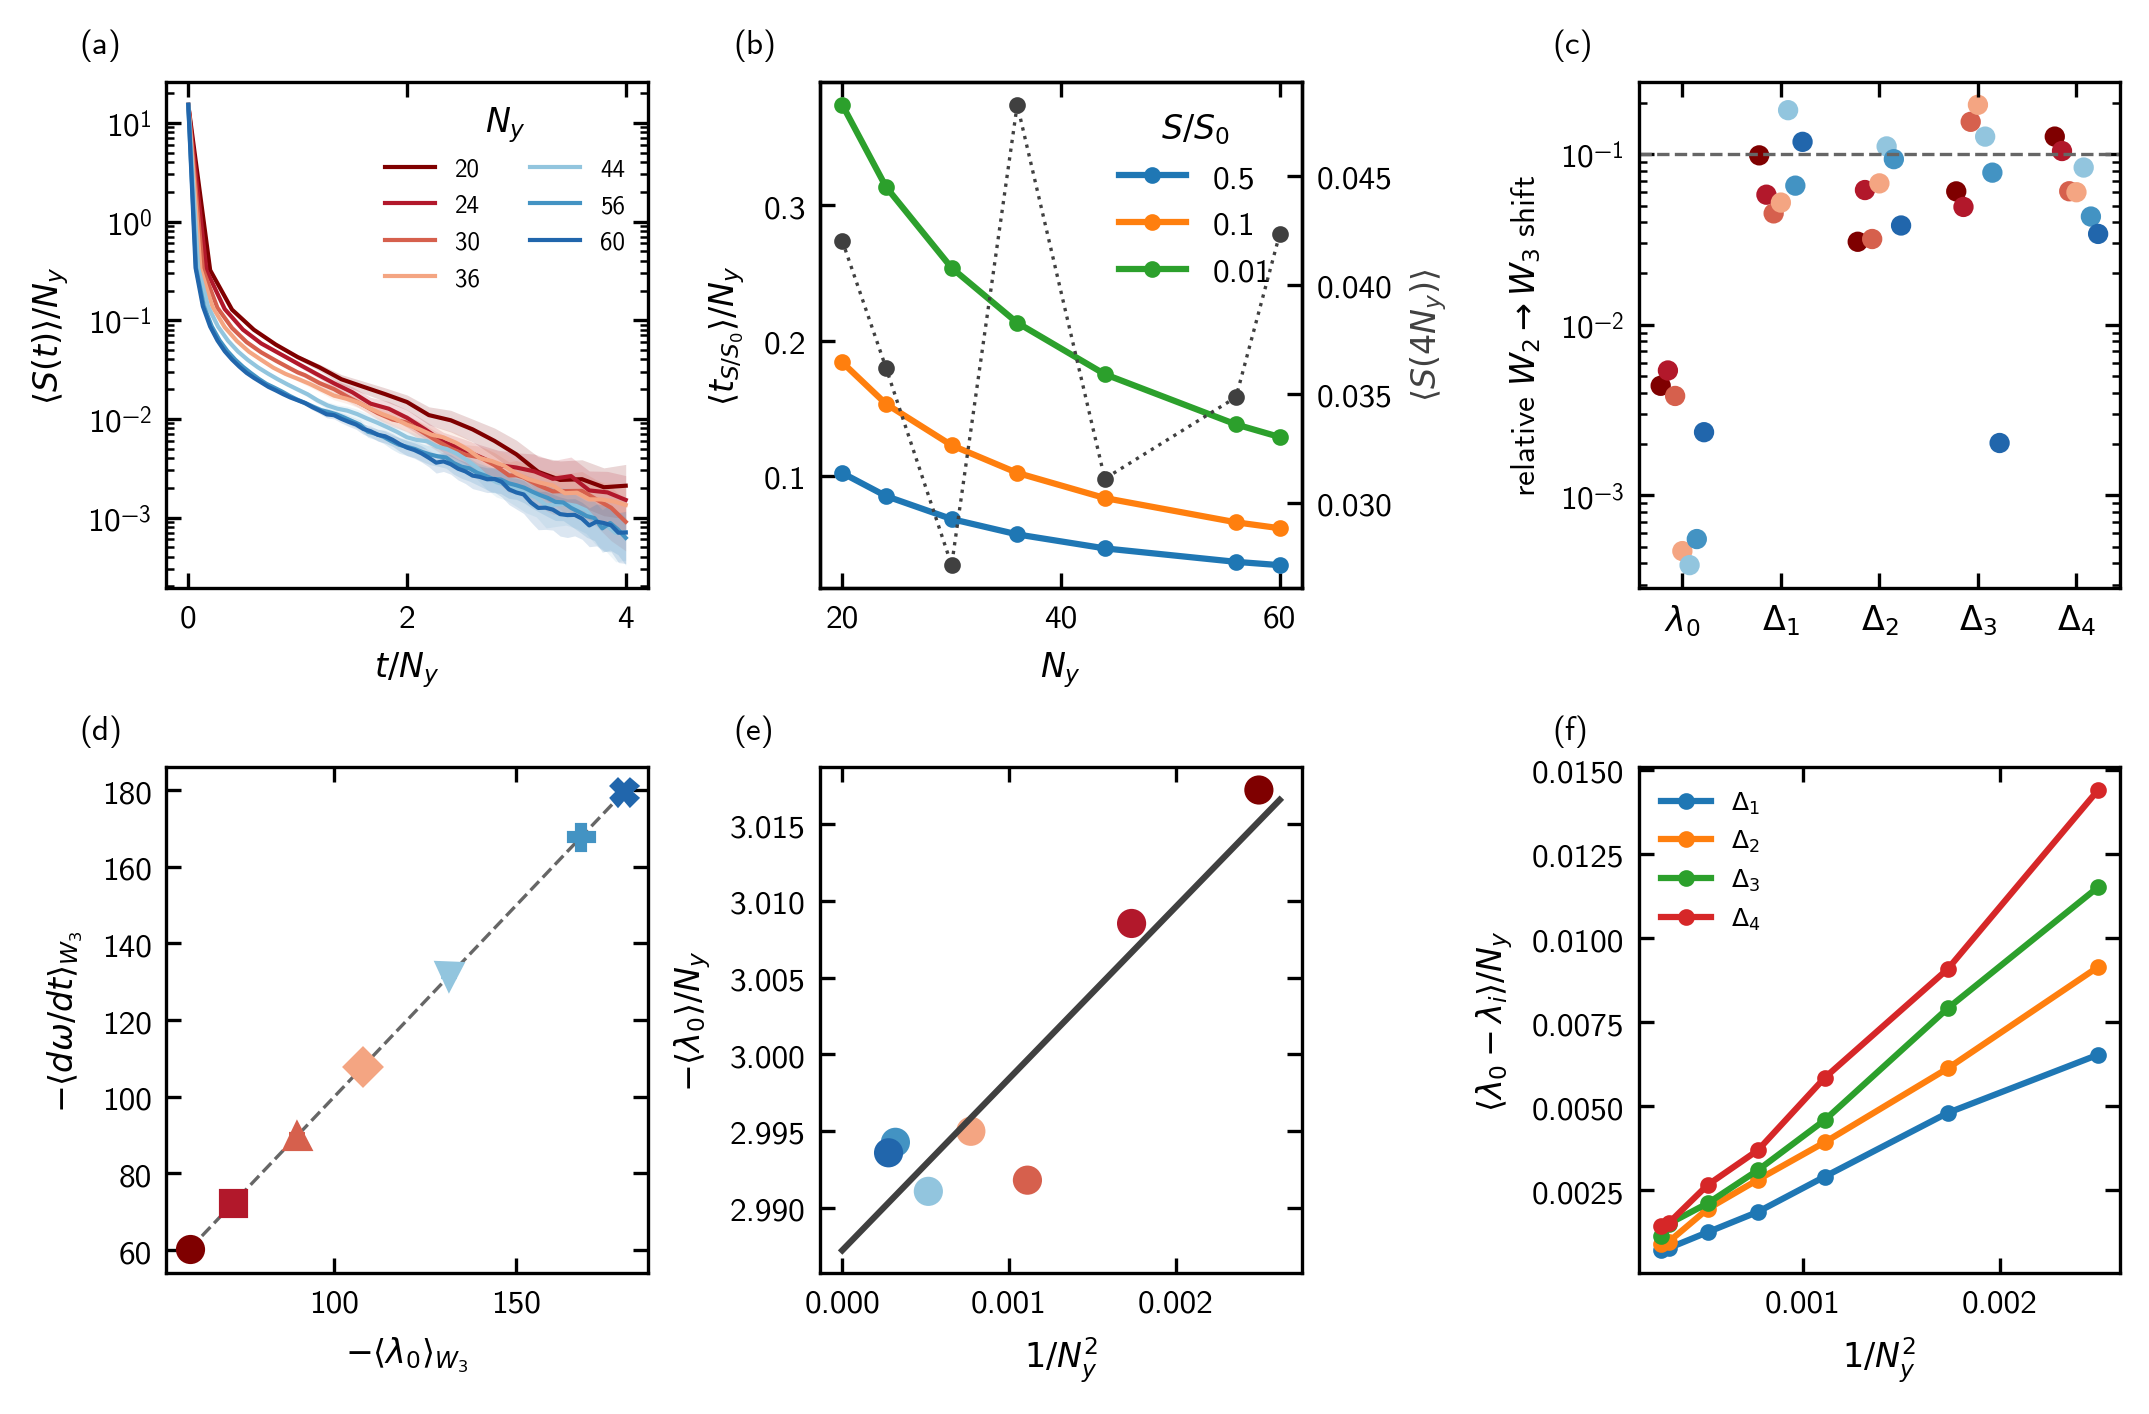
\includegraphics[width=\textwidth]{figure_assets/dynamical_critical_main.png}
\caption{Primary dynamical-critical results. (a) Entropy-density collapse with whole-trajectory bootstrap intervals.
(b) Sample-wise purification times and endpoint residual entropy. (c) Relative $W_2\to W_3$ shifts.
(d) Same-window record-weight closure. (e) Leading finite-size fit. (f) Ordered-gap densities.
Colors label circumference.}
\end{figure*}

\section{Purification and temporal convergence}
The endpoint entropy is small at every circumference, while the full $S(t)/N_y$ curves provide a direct
descriptive test of $z=1$ scaling. Threshold-crossing times are linearly interpolated on the native
four-cycle grid; an exploratory exponent is withheld unless the three thresholds and omitted-smallest-size
fit agree. The combined late temporal gate is \textbf{failed}. This gate requires
the paired $W_2\to W_3$ confidence interval to contain zero, a mean shift below 10\%, and at least 95\%
resolved trajectories for every reported metric.

\section{Record closure and boundary localization}
The leading reconstructed level is compared with $d\omega/dt$ in the same fit window. The endpoint ratio
$-\omega(T)/T$ is retained only as a finite-depth diagnostic. The $W_3$ record-closure ledger
\textbf{passed} its one-percent criterion across all sizes. The first four soft modes
are analyzed only through their aggregate subspace density and aggregate weight near both walls. This avoids
nonphysical labels under rotations in nearly degenerate eigenspaces.

\section{Finite-size coefficients and claim gates}
The late-window leading density is fit to
\begin{equation}
 -\lambda_0/N_y=f_\infty+A_0/N_y^2,
\end{equation}
with $1/N_y^4$ and successive $N_{y,\min}=24,30,36$ sensitivity fits. The primary result is
$A_0=11.19$ with 95\% interval
$[-4.148,27.04]$.
The derived $\alpha c_{\rm eff}=-6A_0/\pi$ is
\textbf{not released}; release requires the physical sign, bootstrap
significance, temporal stability, and below-20\% fit sensitivity simultaneously. The same rules, plus
resolved-sample gates, apply to $\alpha x_i=A_i/(2\pi)$. Released ordered gaps: none.
No conformal operator names are assigned because momentum, charge-sector, and two-wall symmetry labels were
not saved.

\begin{figure*}[t]
\centering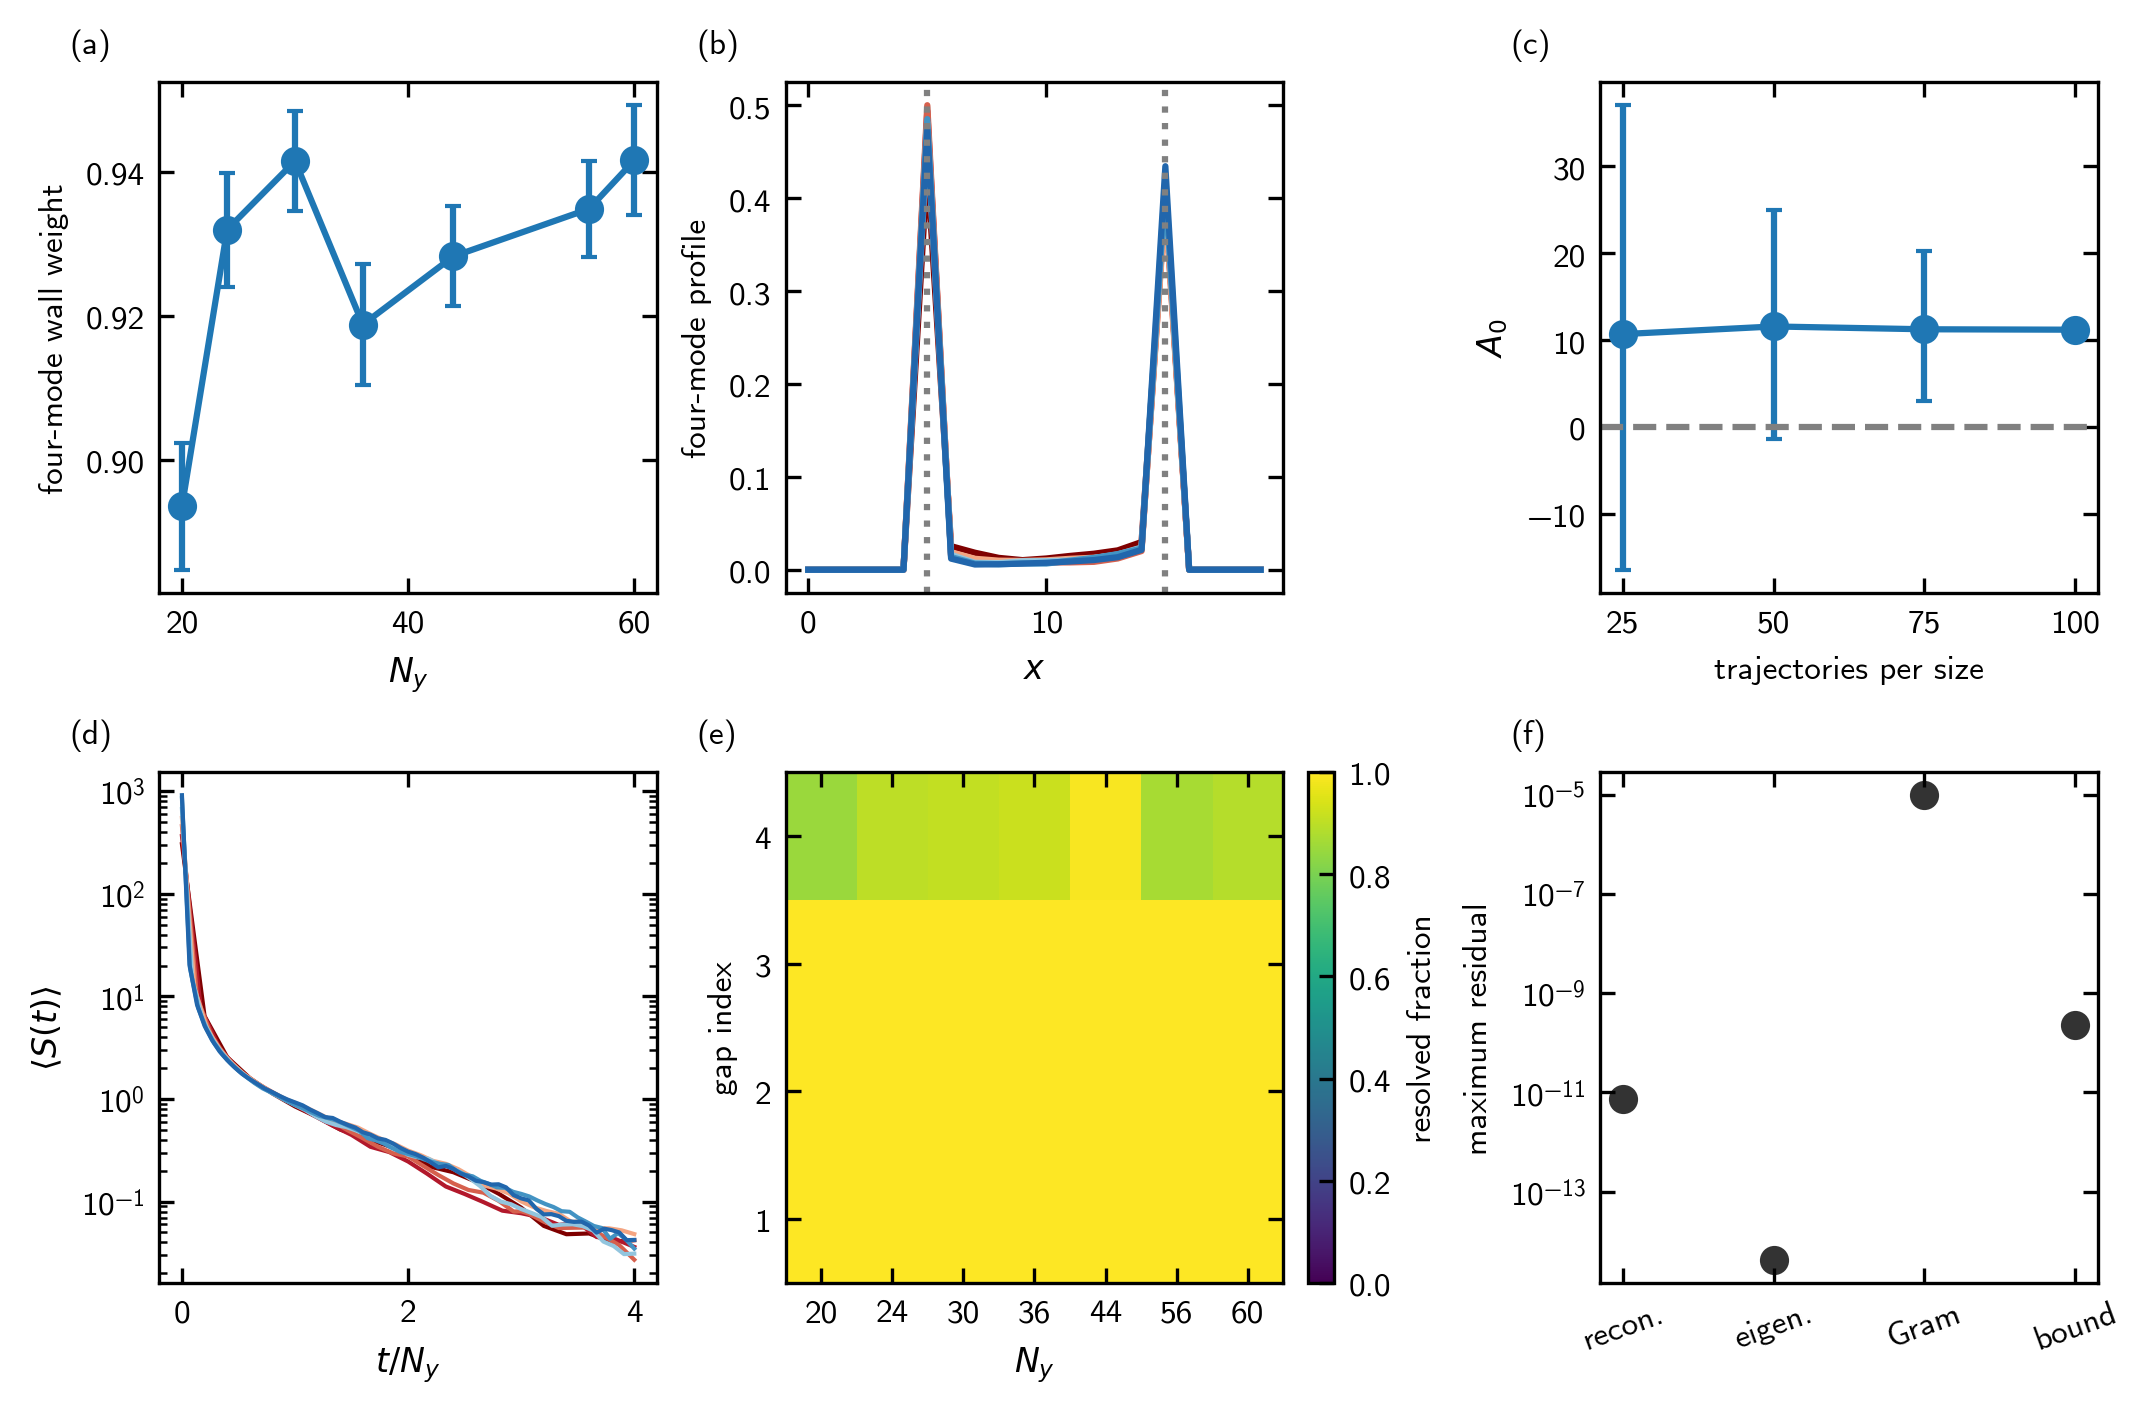
\includegraphics[width=\textwidth]{figure_assets/dynamical_critical_diagnostics.png}
\caption{Diagnostics. (a,b) Aggregate four-mode wall localization and transverse profile.
(c) Random without-replacement sample convergence. (d) Unnormalized entropy dynamics. (e) Resolved fractions.
(f) Maximum numerical residuals.}
\end{figure*}

\section{Relation to earlier ensembles}
The earlier $2N_y$ pilot and the independent three-size $4N_y$ purification campaign are compared only at
the summary-ledger level. Their trajectories are never pooled with this primary seven-size campaign.

\section{Conclusion}
The completed data validate the Gaussian many-body spectral reconstruction, deep-time purification,
same-window record closure, and boundary localization. Any failed gate remains explicit in the accompanying
CSV and JSON ledgers; an unphysical or unstable coefficient is not converted into a claim about
$c_{\rm eff}$ or absolute operator dimensions.
\end{document}
